% 2007 年上海卷文科第 11 题：等半径圆与直线 l 相切于 A、B。
% 以两圆的上方公共点 C 连接圆弧 AC、CB。曲线按原图作对称示意，不用于测量半径。
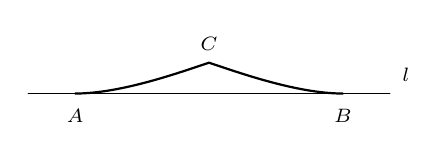
\begin{tikzpicture}[x=1.7cm,y=.7cm,line cap=round,line join=round,
  every node/.style={font=\scriptsize}]
  \coordinate (A) at (0,0);
  \coordinate (B) at (2,0);
  \coordinate (C) at (1,.56);

  \draw[line width=.45pt] (-.35,0)--(2.35,0);
  \draw[thick] (A) .. controls (.35,0) and (.8,.4) .. (C);
  \draw[thick] (C) .. controls (1.2,.4) and (1.65,0) .. (B);

  \node[below=2pt] at (A) {$A$};
  \node[above=1pt] at (C) {$C$};
  \node[below=2pt] at (B) {$B$};
  \node[above right=1pt] at (2.35,0) {$l$};
\end{tikzpicture}
